\chapter*{Búsqueda binaria}
\markboth{Búsqueda binaria}{Búsqueda binaria}
\addcontentsline{toc}{chapter}{Búsqueda binaria}

Esta técnica es una de las más poderosas e importantes en la informática. Es una forma muy eficiente de hacer búsquedas que nos permite resolver problemas antes imposibles.

Utilizada en muchas aplicaciones, nos permite resolver problemas donde una búsqueda completa tardaría miles de millones de años en menos de un segundo. Y esta impresionante herramienta ahora será tuya.

La búsqueda binaria difiere de la completa al evitar revisar absolutamente todas las opciones del espacio de búsqueda. Si no, lo que hace es que en cada paso logra descartar la mitad del espacio de búsqueda al darse cuenta que la respuesta no está allí.

Porque en cada paso va descartando la mitad de las opciones, llega a una única opción (la respuesta si esta existe) en muy poco tiempo. Mientras que la búsqueda completa va eliminando opciones de una en una.

Comparemos un ejemplo de la búsqueda completa vs la binaria, si tuviéramos \(128\) candidatos. 

\begin{center}
	\begin{tabular}{|c|c|c|}
		\hline
		\multirow{2}{*}{\shortstack{Número\\ de pasos}} & \multicolumn{2}{c|}{Candidatos restantes} \\
		\cline{2-3}
		 & Completa & Binaria \\
		\hline
		0 & 128 & 128  \\		
		\hline
		1 & 127 & 64  \\		
		\hline
		2 & 126 & 32  \\
		\hline
		3 & 125 & 16  \\
		\hline
		4 & 124 & 8  \\
		\hline
		5 & 123 & 4  \\
		\hline
		6 & 122 & 2  \\
		\hline
		7 & 121 & 1  \\
		\hline
		8 & 120 &   \\	
		\multicolumn{3}{c}{
	\begin{LARGE}
	
		\(\cdots\)
		
	\end{LARGE} 
	}\\
		125 & 3 &  \\		
		\hline
		126 & 2 &  \\		
		\hline
		127 & 1 &  \\
		\hline
	\end{tabular}
\end{center}

Como vemos, búsqueda binaria pudo reducir los candidatos a solo uno con siete pasos, mientras que la búsqueda completa requirió de 127.

El motivo por el cuál la búsqueda binaria es tan efectiva, es que realiza \(\lceil log_2(candidatos) \rceil\) pasos \footnote{\(\lceil log_2(A) \rceil \) significa: techo del logaritmo base dos de A.\\ Recordemos que \(log_2(A)=x\) significa que \(2^x=A\).\\ Y el techo nos dice que tomemos el menor entero que sea mayor igual que el valor de adentro, por ejemplo:. \(\lceil 3.12 \rceil =4\)}. Esto es porque \(\lceil log_2 \rceil \) nos permite calcular cuantas veces podemos dividir un número entre dos hasta que sea 1.

Veamos un ejemplo que se puede resolver con búsqueda binaria.

\section*{Ejemplo 3.1}
\addcontentsline{toc}{section}{Ejemplo 3.1}

Javier es un granjero y esta cansado de que sus animales siempre huyan de su terreno, por lo que ha decidido poner una reja al rededor de todo el terreno.

Sin embargo, Javier no sabe cuantos metros de reja va a necesitar y te ha contratado para que tu le digas esto. 

Lo que él si sabe es que el tiene forma cuadrada con lados de longitud entera, además recuerda que este mide \(A\) metros cuadrados de área.

Ayuda a Javier para que sepa cuanta reja necesita.

\subsection*{Entrada}
Un entero \(A\), el tamaño del terreno en metros cuadrados.
\subsection*{Salida}
Un entero indicando cuantos metros de reja necesita para rodear todo el terreno. 

\subsection*{Ejemplos}
\begin{casebox2}
	\scase{36}{24}
	\scase{100}{40}
	\scase{1}{4}
\end{casebox2}

\subsection*{Límites}
\begin{plimits}
	\item \(1\leq A \leq 10^{18}\)
\end{plimits}
\subsection*{Subtareas}
\begin{plimits}
	\item (35 pts) \(1\leq A \leq 10^9\)
	\item (65 pts) Sin restricciones adicionales
\end{plimits}

\subsection*{Solución}
Como siempre, antes de leer la solución te invitamos a que intentes el problema.


En este problema nos piden de que dado el área de un cuadrado, imprimamos el perímetro. Por esto, recordemos las formulas del cuadrado.
\[Per\acute{i}metro=4\times Lado \]
\[\acute{A}rea=Lado\times Lado \]

Entonces, si encontramos el lado que nos de el área de entrada, podremos encontrar el perímetro.

Para este problema vamos a ver dos estrategias para resolverlo, la de búsqueda lineal y la binaria.

Comencemos con la que ya deberíamos estar familiarizada, usemos búsqueda lineal.

\subsubsection*{Búsqueda lineal}
Entonces, buscaremos el entero \(L\) de entre todos los posibles, que cumpla que \(A=4\times L\). Para esto, podremos ir probando del \(1\) en adelante hasta encontrar el que cumpla.

\begin{lstlisting}
	long long L=1;
	while (L*L != A) {
		L++;
	}
\end{lstlisting}

Esto itera por todos los enteros del \(1\) a la respuesta que es \(\sqrt{A}\). Por lo tanto, su complejidad es \(O(\sqrt{A})\). Lo cual corre para la subtarea de 35 puntos, pero no para el límite completo de \(10^{18}\).

\subsubsection*{Búsqueda binaria}
Ahora resolvamos el problema utilizando búsqueda binaria.

Definamos nuestro espacio de búsqueda, ¿cuáles valores puede ser \(L\)? y si lo pensamos puede ser desde \(1\) hasta \(10^9\). Porque \(10^9\times 10^9=10^{18}\) y de los límites sabemos que \(1\leq A\leq 10^{18}\).

Entonces queremos encontrar la respuesta que esta entre \(1\) y \(10^9\), hagamos una función que logre esto llamada buscar que reciba el rango de donde esta la respuesta.

\begin{lstlisting}
	//Encuentra L tal que L*L=A, sabiendo que a<=L<=b.
	long long buscar(long long a, long long b, long long A);
\end{lstlisting}

Ahora tenemos \(10^9\) candidatos donde encontrar la respuesta y queremos reducirlo a la mitad. 

Para esto podemos ver que sucede con \(5\times10^8\). 

Si resulta que \((5\times10^8)\times(5\times10^8) <A\), entonces sabemos que cualquier valor menor igual que \(5 \times 10^8\) no funcionará porque es demasiado pequeño. Por lo tanto la respuesta debe estar entre \(5\times 10^8 +1\) y \(10^9\) y los candidatos se redujeron a la mitad.

Pero si en vez sucede que \((5\times10^8)\times(5\times10^8) >=A\), entonces sabremos que cualquier valor más grande que \(5\times 10^8\) nos dará valores más grandes que \(A\) y por lo tanto la respuesta no estará allí. Ahora nuestros candidatos son los números entre \(1\) y \(5\times 10^8\), reduciendo los valores que podrían ser la respuesta a la mitad.

Y de hecho, si en general, la respuesta esta entre \(a\) y \(b\), nos convendrá preguntar por el punto medio \((a+b)/2\), que nos reducirá el espacio a la mitad.

Una vez que redujimos el rango de la búsqueda, tendremos que encontrar la respuesta en ese nuevo rango, y para esto podemos hacer recursión.

De forma que ahora tenemos:
\begin{lstlisting}
	long long buscar(long long a, long long b, long long A) {
		long long m =(a+b)/2;
		if (m*m < A) {
			return buscar(m+1, b, A);
		} else {
			return buscar(a, m, A);
		}
	} 
\end{lstlisting}

Ahora, lo que le falta a esa recursión es una condición de paro, saber cuando ya termino y encontramos la respuesta.

Podremos ver que habremos encontrado la respuesta cuando ya estemos seguros de cual es esta. Y esto sucede cuando nuestro rango solo incluye un valor, es decir, cuando \(a==b\) se cumpla.

\begin{lstlisting}
	long long buscar(long lonng a, long long b, long long A) {
		if (a==b)
			return a;
		long long m=(a+b)/2;
		if (m*m<A) {
			return buscar(m+1, b, A);
		} else {
			return buscar(a, m, A);
		}
	}
\end{lstlisting}

Y con esto, tenemos que \verb|L=buscar(1, 1000000000, A)|.

Ahora, la complejidad de esto es \(O(log(\sqrt{A}))\), lo cual corre perfectamente para \(10^{18}\).

\paragraph{Nota:} En este problemas también se pudo haber usado \verb|L=sqrt(A)| con la librería \verb|<math.h>| que calcula el valor rápidamente, pero se uso búsqueda binaria para ejemplificar.


\section*{Ejemplo 3.2}
\addcontentsline{toc}{section}{Ejemplo 3.2}
Se te da un arreglo \(A\) de \(N\) enteros diferentes. El arreglo estará en orden creciente, es decir, \(A[i] < A[i+1]\).

Deberás responder \(T\) preguntas:

Cada pregunta consistirá de un entero \(q_i\) y tu deberás imprimir el índice del valor \(q_i\) o \(-1\) si este valor no existe.
\subsection*{Entrada}
El enteros \(N\).

En la siguiente línea: \(N\) enteros separados, los valores del arreglo \(A\).

En la siguiente línea recibirás el entero \(T\).

En las siguientes \(T\) líneas recibirás los valores de cada pregunta.

\subsection*{Salida}
Imprime la respuesta cada pregunta en una línea en el mismo orden que el de lectura.

\subsection*{Ejemplo}
\begin{casebox2}
	\scase{
		7\\
		2 5 6 7 8 9 10\\
		5\\
		2\\
		6\\
		4\\
		10\\
		5\\
	}
	{
		0\\
		2\\
		-1\\
		6\\
		1		
	}
\end{casebox2}
\subsection*{Límites}
\begin{plimits}
	\item \(1\leq N,T \leq 10^5 \)
	\item \(1\leq A[i], q_i \leq 10^9 \)
\end{plimits}

Enlace: TODO

\subsection*{Solución}
Esta ocasión nos piden encontrar el indice de un valor en un arreglo ordenado. Ya hemos visto como hacerlo con búsqueda lineal:

\begin{lstlisting}
	int indice(int q) {
		for (int i =0; i < N;i++) 
			if (A[i]==q)
				return i;
		return -1;
	}
\end{lstlisting}

Sin embargo, esto no corre en tiempo ya que la complejidad es \(O(N)\) por pregunta, siendo en total \(O(TN)\) y como \(TN=10^{10}\), obtendremos TLE.

Pero veamos que podemos usar búsqueda binaria. ya que al preguntar por una posición de en medio y discernir si tenemos que buscar adelante o atrás.

\begin{lstlisting}
	int binaria(int a, int b, int q) {
		if (a>b)
			return -1;
		int m =(a+b)/2;
		if (A[m]==q)
			return m;
		if (A[m]<q) {
			return binaria(m+1, b, q);
		} else {
			return binaria(a, m-1, q);
		}		
	}
	int indice(int q) {
		return binaria(0, N-1, q);
	}
\end{lstlisting}

La nueva complejidad ahora es \(O(logN)\) por pregunta, en total \(O(TlogN)\)

\section*{Dificultades}
\addcontentsline{toc}{section}{Dificultades}
Ya vimos que la búsqueda binaria tiene una ventaja enorme sobre la búsqueda lineal ya que resuelve el problema en un tiempo mucho menor.

Pero tristemente, no siempre es posible aplicar la búsqueda binaria. Hay veces en que las que no se puede descartar fácilmente la mitad de los candidatos.

Un caso donde puede suceder sería en el ejemplo anterior si el arreglo no estuviese ordenado. En ese caso no podríamos hacer el truco de solo revisar adelante si \(A[m]<q\) ya que no nos da suficiente información esa pregunta para eliminar todos los valores de \(0\) a \(m\).

Por supuesto, el problema anterior tiene corrección para que la búsqueda binaria siga funcionando y muchas veces esto es parte del problema, ¿cómo hago la binaria aquí? Pero hay otras veces que es imposible, o al menos, más allá de los conocimientos actuales.

En esos casos, no quedará de otra más que hacer búsqueda completa o usar una técnica diferente a búsqueda.

Otro ejemplo donde la búsqueda binaria no se puede utilizar es en encontrar el primer divisor que no sea 1 de un entero.
\newpage
\section*{Problemas de práctica}
\addcontentsline{toc}{section}{Problemas de práctica}

\paragraph{Problema 3.1} Adivina el número que esta pensando OmegaUp.

Deberás implementar una función \verb|void adivina(long long a, long long b)| que descubra el número \(s\) que OmegaUp esta pensando. Se cumplirá que \(a\leq s\leq b\).

Para adivinar el número podrás llamar a la función \verb|long long pista(long long x)|.

Esta función regresará:
\begin{plimits}
	\item \verb|-1| si el número que piensa OmegaUp es menor que \(x\).
	\item \verb|0| si el número que piensa OmegaUp es \(x\).
	\item \verb|1| si el número que piensa OmegaUp es mayor que \(x\).
\end{plimits} 

La ultima llamada a pista debe ser con el número que OmegaUp esta pensando.

\subsubsection*{Límites}
\begin{plimits}
	\item \(-2^{61}\leq a,b \leq 2^{61}\)	
\end{plimits}
\subsubsection*{Evaluación}
Tu puntuación será en base a la cantidad de llamadas que hagas a la función \verb|long long pista(long long x)| de la siguiente manera:
\begin{plimits}
	\item 100\% si haces a lo más \(log(b-a+1)\)llamadas
	\item 50\% si haces a lo más \(2log(b-a+1)\)llamadas
	\item 0\% si haces más de \(2log(b-a+1)\)llamadas
\end{plimits}

Enlace: \omegalink{COMI-Adivina-el-numero}

NOTA: Este es un problema interactivo, si no conoces como trabajar con estos, ve la página: \pageref{interactivos}

\problembreak

\paragraph{Problema 3.2} Sho colecciona juegos de dominó y quiere jugar.

Pero los dominós de Sho son un poco especiales, ya que son k-dominós. El dominó tradicional es del tipo 6-dominó, porque tiene números del \(0\) al \(6\), con un total de 28 fichas.

Entonces, un k-dominó tendrá números del \(0\) al \(k\). Con una ficha por cada par posible de números, incluyendo las mulas (mula es el mismo número emparejado consigo mismo).

Las fichas del 6-dominó son:

\begin{center}
		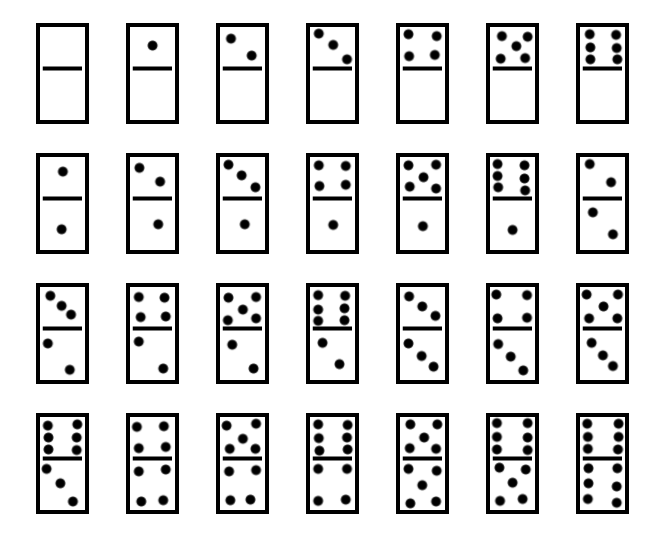
\includegraphics[scale=0.4]{domino6}
\end{center}

Y las del 2-domino son las siguientes seis:
\begin{center}
	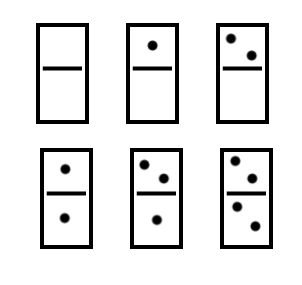
\includegraphics[scale=0.4]{domino2}
\end{center}

Sho quiere jugar con al menos \(N\) fichas, pero como después de jugar tiene que guardar, quiere usar el dominó con menor cantidad de fichas que tenga por lo menos \(N\) fichas. 

Dado \(N\), encuentra el valor de \(k\) para el k-dominó que le sirve a Sho.

\subsubsection*{Ejemplo}
\begin{casebox2}
	\scase{30}{6}
	\scase{6}{2}
	\scase{1000}{44}
\end{casebox2}

\subsubsection*{Límites}
\begin{plimits}
	\item \(1\leq N \leq 10^{18}\)
\end{plimits}

Enlace: TODO

\section*{Función de validación}
\addcontentsline{toc}{section}{Función de validación}
Igual que en búsqueda lineal podíamos agregar funciones más complicadas a la hora de buscar la respuesta, lo mismo sucede en búsqueda binaria. A veces requeriremos de más código que una simple comparación para saber en cual mitad esta la respuesta.

Veamos unos ejemplos.


\section*{Ejemplo 3.3}
\addcontentsline{toc}{section}{Ejemplo 3.3}
TODO: PENSAR UN PROBLEMA CON FORMULA MAS COMPLICADA

\section*{Ejemplo 3.4}
Karel ha comprado una bicicleta eléctrica con la que planea completar un recorrido. El recorrido se puede ver como \(N\) colinas en línea recta tal que la \(i\)-ésima colina tiene altura \(h_i\). Karel comienza en la colina hasta la izquierda y quiere terminar en la ultima colina de hasta la derecha.

Cuando Karel sube un metro gasta \(1\) unidad de energía, mientras que bajar un metro recupera \(1\) unidad de altura. Si Karel en algún momento necesita subir, pero su batería tiene 0 de energía, Karel se quedará atorado y no terminará el recorrido.

Por suerte al inicio hay una estación de recarga donde Karel puede recargar su bicicleta. Como nota, la batería tiene capacidad \(R\) y jamás podrá almacena más energía que \(R\).

Actualmente Karel tiene \(0\) de energía, Determina cuál es la menor cantidad de energía que es necesaria recargar al inicio para completar el recorrido. O determina si es imposible hacer el recorrido con la bicicleta de Karel.

\subsubsection*{Entrada}
La primera línea tiene dos enteros, el valor de \(N\) y \(R\).

En la siguiente línea vienen \(N\), enteros separados por espacios, siendo la altura de las colinas de izquierda a derecha. Recuerda que Karel comienza en la primera colina y quiera terminar en la última.
\subsubsection*{Salida}
Un entero, representando la menor cantidad de energía necesaria para completar el recorrido. Si Karel no puede completar el recorrido, imprime \(-1\).

\subsubsection*{Casos ejemplo}
\begin{casebox3}	
	\ecase{
		6 8\\
		4 6 3 5 7 
	}
	{3}
	{
		Karel inicia con 3 de energía, moverse de   \\
		la primera a la segunda colina le toma 2,  \\
		ahora tiene 1.\\
		Luego avanza y se recarga 3,\\
		ahora tiene 4.\\
		Después continua y se consume 2, ahora tiene 2. \\
		Vuelve a avanzar quedándose con 0 de energía. \\		
		Pero luego avanza y se recarga a 5. \\
		Finalmente avanza para termina con 5. \\
	}
	\ecase{
		5 6\\
		1 10 1 2 0
	}
	{-1}
	{}
	\hline
\end{casebox3}	

\subsubsection*{Límites}
\begin{plimits}
	\item \(2\leq N, R \leq 10^5\)
	\item \(0\leq h_i\leq 10^9\)
\end{plimits}

Fuente: OMIS online 2022.

Enlace: [TODO]

\section*{Solución}
Este problema 1.6 de búsqueda lineal con validación en la página \pageref{bicicleta}, si no sabes resolverlo con búsqueda lineal para los límites de allí, primero descubre esa solución.

Esta vez, los límites son más estrictos, de forma que la solución estándar con búsqueda lineal no funciona, pero veamos cual es porque nos será útil.
\\

La respuesta siempre estará entre \(0\)  y\(R\). La búsqueda lineal funciona de la siguiente manera.
\begin{lstlisting}
	int respuesta=-1;
	for (int e=0; e<=R; e++) {
		if (funciona(e)) {
			respuesta=e;
			break;
		}
	}
\end{lstlisting}

Y la función \verb|bool funciona(int e)| te regresa verdadero si Karel puede completar el recorrido comenzando con \(e\) de energía.

Esta función simplemente simula el recorrido para ver si Karel se atora en algún momento. Se ve de la siguiente forma:

\begin{lstlisting}
	bool funciona(int e) {
		for (int i = 1; i <N; i++){
			e-=A[i]-A[i-1];
			if (e > R) 
				e=R; //Limita la energia
			if (e < 0)
				return false;			
		}
		return true;
	}
\end{lstlisting}

La función \verb|funciona()| tiene una complejidad de \(O(N)\) y como es llamada en \(R\) valores, la complejidad total es \(O(RN)\).

Pero ahora veamos dos hechos importantes:
\begin{itemize}
	\item Si funciona(m) cumple, también lo hará cualquier valor mayor que \(m\).
	\item Si funciona(m) falla, también lo hará cualquier valor menor que \(m\).
\end{itemize}

Es decir, se ve de la siguiente forma:

TODO PONER IMAGEN AQUI

Esto hace que podamos hacer búsqueda binaria para encontar el primer SI.

El código se verá como:

\begin{lstlisting}
	int a=0,b=R;
	while(a!=b) {
		int m=(a+b)/2;
		if (funciona(m)) {
			b=m;
		} else {
			a=m+1;
		}
	}
	int respuesta=-1;
	if (funciona(a))
		respuesta=a;
\end{lstlisting}

Ahora, recordemos que la complejidad de la búsqueda binaria es \(O(logR)\), pero en cada paso de la búsqueda estamos llamando a \verb|funciona()| que tiene complejidad \(O(N)\), por lo tanto, la complejidad total es \(O(NlogR)\).

\section*{Problemas de práctica}
\addcontentsline{toc}{section}{Problemas de práctica}
TODO: PONER PROBLEMAS DE PRACTICA AQUI
\paragraph{Problema 3.3} Palomitas CF\\

\problembreak

\paragraph{Problema 3.4} Dado un arreglo \(A\) de \(N\) enteros, determina si existe un subcadena que sume \(K\).

Una subcadena es cualquier subarreglo de elementos continuos.

\newpage
\section*{Búsqueda en los reales}
\addcontentsline{toc}{section}{Búsqueda en los reales}

Hay veces en la que no estamos buscando un valor entero, si no en vez querremos encontrar un valor real a cierta precisión.

El problema dirá algo por el estilo de: imprime la respuesta con precisión de \(10^{-6}\), esto quiere decir que tu respuesta no debe estar alejada de la solución por más de \(10^{-6}\).

Para estos problemas debes cambiar la condición de paro de \(a==b\), por \(b-a < precision\). Aunque en realidad, recomiendo poner una precisión un poco más ajustada ya que no tiende a aumentar mucho el costo.

De forma que ahora la binaria se verá como:

\begin{lstlisting}
	double a =0, b=1e9;
	double epsilon = 1e-8;
	while(b-a>= epsilon) {
		double m = (a+b)/2;
		if (funciona(m)) {
			b=m;
		} else {
			a=m;
		}
	}
\end{lstlisting}

\section*{Ejemplo 3.5}
\addcontentsline{toc}{section}{Ejemplo 3.5}
Calcula la raíz cuadrada de un número A con precisión absoluta de \(10^{-4}\).
\subsection*{Ejemplo}
\begin{casebox2}
	\scase{10}{3.1622}
	\scase{16}{4.0000}
\end{casebox2}
\subsection*{Límites}
\begin{plimits}
	\item \(1\leq A \leq 10^9\)
\end{plimits}
\subsection*{Solución}
Usamos las mismas observaciones que usamos para el ejemplo 3.1, pero esta vez lo haremos con double y nos detenemos basados en una precisión.
\begin{lstlisting}
	double raiz(double A) {
		double a=0, b=A;
		while (b-a >= 1e-5) {
			double m=(a+b)/2;
			if (m*m < A) {
				a=m;
			} else {
				b=m;
			}
		}
		return a;
	}
\end{lstlisting}

\newpage
\section*{Problemas de practica}
\addcontentsline{toc}{section}{Problemas de práctica}
\paragraph{Problema 3.5} Fernando ha adquirido un gusto por las carreras de coches en la fórmula \(\pi\).

En este deporte, los coches recorren una pista recta que mide \(L\) metros de longitud. Además, dependiendo de resultados anteriores el coche \(i\) inicia con \(x_i\) metros de ventaja.

Como Fer es un aficionado muy dedicado, se ha percatado de que cada coche se moverá hacia la meta con una velocidad constante, en concreto, el .

\problembreak

\paragraph{Problema 3.6} Foto

\omegalink{carretera}
